% mnras_template.tex
%
% LaTeX template for creating an MNRAS paper
%
% v3.0 released 14 May 2015
% (version numbers match those of mnras.cls)
%
% Copyright (C) Royal Astronomical Society 2015
% Authors:
% Keith T. Smith (Royal Astronomical Society)

% Change log
%
% v3.0 May 2015
%    Renamed to match the new package name
%    Version number matches mnras.cls
%    A few minor tweaks to wording
% v1.0 September 2013
%    Beta testing only - never publicly released
%    First version: a simple (ish) template for creating an MNRAS paper

%%%%%%%%%%%%%%%%%%%%%%%%%%%%%%%%%%%%%%%%%%%%%%%%%%
% Basic setup. Most papers should leave these options alone.
\documentclass[a4paper,fleqn,usenatbib]{mnras}

% MNRAS is set in Times font. If you don't have this installed (most LaTeX
% installations will be fine) or prefer the old Computer Modern fonts, comment
% out the following line
\usepackage{newtxtext,newtxmath}
% Depending on your LaTeX fonts installation, you might get better results with one of these:
%\usepackage{mathptmx}
%\usepackage{txfonts}

% Use vector fonts, so it zooms properly in on-screen viewing software
% Don't change these lines unless you know what you are doing
\usepackage[T1]{fontenc}
\usepackage{ae,aecompl}


%%%%% AUTHORS - PLACE YOUR OWN PACKAGES HERE %%%%%

% Only include extra packages if you really need them. Common packages are:
\usepackage{graphicx}	% Including figure files
\usepackage{amsmath}	% Advanced maths commands
\usepackage{amssymb}	% Extra maths symbols
\usepackage{xspace}
\usepackage{subfig}
\usepackage{tabularx}
\usepackage{hyperref}


%%%%%%%%%%%%%%%%%%%%%%%%%%%%%%%%%%%%%%%%%%%%%%%%%%

%%%%% AUTHORS - PLACE YOUR OWN COMMANDS HERE %%%%%

% Please keep new commands to a minimum, and use \newcommand not \def to avoid
% overwriting existing commands. Example:
%\newcommand{\pcm}{\,cm$^{-2}$}	% per cm-squared
\newcommand{\sgx}{\textsc{s}g\textsc{xb}\xspace}
\newcommand{\sfxt}{\textsc{sfxt}}
\newcommand{\sg}{Sg\xspace}
\newcommand{\co}{CO\xspace}
\newcommand*{\hmxb}{\textsc{hmxb}\@\xspace}
\newcommand*{\ns}{\textsc{ns}\@\xspace}
\newcommand*{\eg}{e.g.\@\xspace}
\newcommand*{\ie}{i.e.\@\xspace}
\newcommand*{\aka}{a.k.a. \@\xspace}


%%%%%%%%%%%%%%%%%%%%%%%%%%%%%%%%%%%%%%%%%%%%%%%%%%

%%%%%%%%%%%%%%%%%%% TITLE PAGE %%%%%%%%%%%%%%%%%%%

% Title of the paper, and the short title which is used in the headers.
% Keep the title short and informative.
\title[Disc formation in SgXB]{Wind accretion in Supergiant X-ray binaries\\II. Disc formation}

% The list of authors, and the short list which is used in the headers.
% If you need two or more lines of authors, add an extra line using \newauthor
\author[I. El Mellah, A. A. C. Sander, J.O. Sundqvist, R. Keppens]{
I. El Mellah$^{1}$\thanks{E-mail: ileyk.elmellah@kuleuven.be},
A. A. C. Sander$^{2}$,
J.O. Sundqvist$^{3}$,
R. Keppens$^{1}$
\\
% List of institutions
$^{1}$Centre for mathematical Plasma Astrophysics, Department of Mathematics, KU Leuven, Celestijnenlaan 200B, B-3001 Leuven, Belgium\\
$^{2}$Institut f{\"u}r Physik und Astronomie, Universit{\"a}t Potsdam, Karl-Liebknecht-Str. 24/25, 14476 Potsdam, Germany\\
$^{3}$KU Leuven, Instituut voor Sterrenkunde, Celestijnenlaan 200D, B-3001 Leuven, Belgium
}

% These dates will be filled out by the publisher
\date{Accepted XXX. Received YYY; in original form ZZZ}

% Enter the current year, for the copyright statements etc.
\pubyear{2018}

% Don't change these lines
\begin{document}
\label{firstpage}
\pagerange{\pageref{firstpage}--\pageref{lastpage}}
\maketitle

% Abstract of the paper
\begin{abstract}

\end{abstract}

% Select between one and six entries from the list of approved keywords.
% Don't make up new ones.
\begin{keywords}
accretion, accretion discs -- X-rays: binaries -- stars: neutron, supergiants, winds, outflows -- methods: numerical 
\end{keywords}

%%%%%%%%%%%%%%%%%%%%%%%%%%%%%%%%%%%%%%%%%%%%%%%%%%

%%%%%%%%%%%%%%%%% BODY OF PAPER %%%%%%%%%%%%%%%%%%

% ------------------------------------------------
\section{Introduction}
\label{sec:intro}
% ------------------------------------------------


% ------------------------------------------------
\section{Model and numerical method}
\label{sec:model}
% ------------------------------------------------

% - - - - - - - - - - - - - - - - - - - - - - - - 
\subsection{At the orbital scale}
\label{sec:orb_scale}
% - - - - - - - - - - - - - - - - - - - - - - - - 
\subsubsection{General principle}
\label{sec:pple}

\begin{figure}
\centering
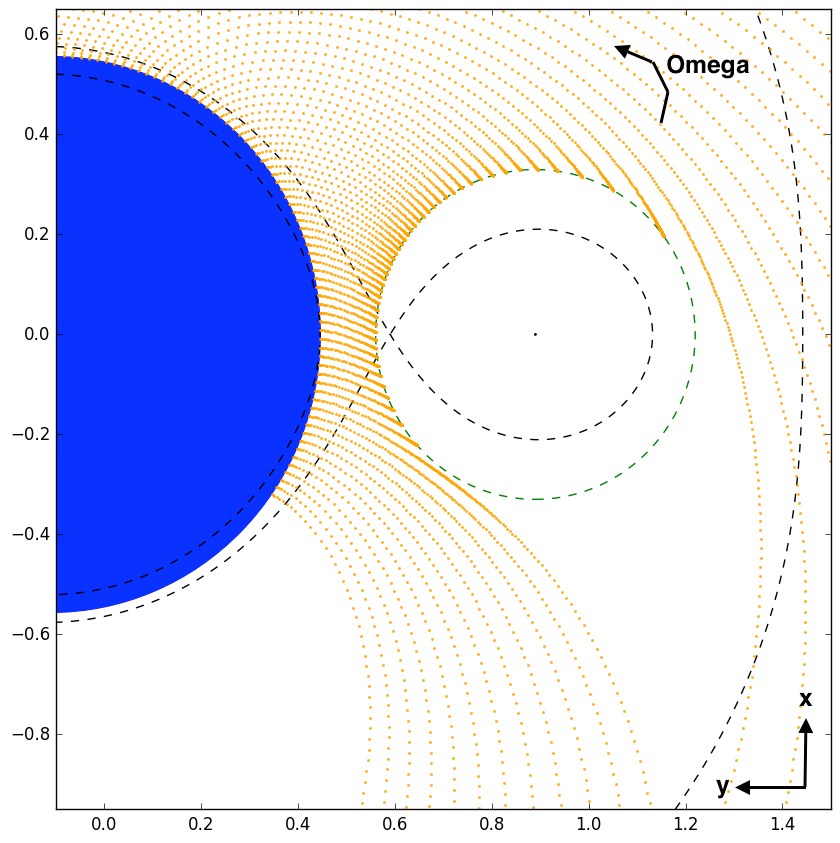
\includegraphics[width=0.9\columnwidth]{Pictures/big_picture.png}
\caption{Computed streamlines (orange dots) from the star (dark blue) to the Roche lobe of the accretor on the right (green dashed circle), in the orbital plane. The black dashed lines represent the critical Roche surface passing by the first Lagrangian point.}
\label{fig:big_picture}
\end{figure} 


\subsubsection{Wind acceleration}
\label{sec:wind_acc}
XXX ANDREAS : would you be able to summarize the principle of your calculation and the way we account for it here?XXX 

\subsubsection{The accretion radius}
\label{sec:acc_rad}

% - - - - - - - - - - - - - - - - - - - - - - - - 
\subsection{Within the Roche lobe of the accretor}
\label{sec:Roche_lobe}
% - - - - - - - - - - - - - - - - - - - - - - - - 

\subsubsection{Equations}
\label{sec:HD_eq}

1 refers to donor star
2 refers to accretor

normalization units

Using the finite volume code \texttt{MPI-AMRVAC} \citep{Xia2017}, we solve the equations of hydrodynamics under their conservative form :

\begin{equation}
\label{eq:eq1}
%\tag{1a}
\partial _t \rho + \boldsymbol{\nabla} \cdot \left( \rho \mathbf{v} \right) = 0
\end{equation}
\begin{equation}
\label{eq:eq2}
%\tag{1b}
\partial _t \left( \rho \mathbf{v} \right) + \boldsymbol {\nabla} \cdot \left( \rho \mathbf{v} \mathbf{v} + P \mathbb{1} \right) = \rho \mathbf{f} - 2 \boldsymbol{\Omega} \wedge \mathbf{v}
\end{equation}
\begin{equation}
\label{eq:eq3}
%\tag{1c}
\partial _t  e  + \boldsymbol{\nabla} \cdot \left[ \left( e + P \right) \mathbf{v} \right] = - \rho \mathbf{v} \cdot \mathbf{f}
\end{equation}
where $\rho$, $\mathbf{v}$, $P$ and $e$ are the mass density, velocity, pressure and total energy density respectively. $\boldsymbol{\Omega}$ is the orbital angular speed vector. $f$ is the modified Roche force per mass unit given by : 

\begin{equation}
\mathbf{f}=\alpha\left( r_1 \right) \frac{q}{r_1^3}\mathbf{r_1} - \frac{1}{r_2^3}\mathbf{r_2} + \frac{1+q}{a^3}\mathbf{r_{\perp}}
\end{equation}

with the mass ratio $q=M_1/M_2$
$\mathbf{r_1}$
$\mathbf{r_2}$
$\mathbf{r_{\perp}}$
$\alpha$ : see section\,\ref{sec:wind_acc}. Encapsulates wind acceleration process and stellar gravity. $-1$ with only gravity, leading to the usual Roche force per unit mass.

The energy equation\,\ref{eq:eq3} is adiabatic. See section\,\ref{sec:cool} for way to account for cooling.
EOS ideal gas monoatomic with an adiabatic index $\gamma=5/3$ with a mean molecular weight set to 1. 



\subsubsection{Cooling}
\label{sec:cool}

Cooling time scale \citep{Schure2009}
Polytropic index $\Gamma$ \citep{Horedt2000}. Physical meaning of $\Gamma$. Bypass the energy equation\,\ref{eq:eq3} where the cooling time scale is XXX times smaller than the dynamical time scale.

Provided the density is high enough, condensation of the hot shocked flow into a disc \citep[][and references therein]{Taam2018} : underlying principle of two component accretion flows models.

\subsubsection{Numerical setup}
\label{sec:num_set}

% - - - - - - - - - - - - - - - - - - - - - - - - 
\subsection{Physical parameters}
\label{sec:params}
% - - - - - - - - - - - - - - - - - - - - - - - - 

\begin{table}
\centering
\caption{Parameters and integrated quantities at the outer edge of the simulation space for the 2 models considered.}
\label{tab:params}
\begin{tabularx}{\linewidth}{c|c|c}
   & LF & HS \\
  \hline
  M$_1$ & \multicolumn{2}{c}{20.2M$_{\odot}$} \\
  R$_1$ & \multicolumn{2}{c}{28.4R$_{\odot}$} \\
  P & \multicolumn{2}{c}{8.964357 days} \\  
  $\dot{\text{M}}_1$ & \multicolumn{2}{c}{6.3$\cdot$10$^{-7}$M$_{\odot}\cdot$yr$^{-1}$} \\
  \hline
  M$_2$ & 1.5M$_{\odot}$  & 2.5M$_{\odot}$  \\
  Boosted & Yes & No  \\
  \hline
  $\dot{\text{M}}_{\text{out}}/\dot{\text{M}}_1$ & XXX & XXX  \\
  $\dot{\text{j}}_{\text{out}}/\dot{\text{j}}_{\text{SL}}$ & XXX & XXX \\
  R$_{\text{circ}}$ / R$_{\text{mag}}$ & XXX & XXX \\
\end{tabularx}
\end{table}


% ------------------------------------------------
\section{Results}
\label{sec:res}
% ------------------------------------------------

% - - - - - - - - - - - - - - - - - - - - - - - - 
\subsection{Inhomogeneity and asymmetry of the inflow}
\label{sec:asymm}
% - - - - - - - - - - - - - - - - - - - - - - - - 

\begin{figure*}
\centering
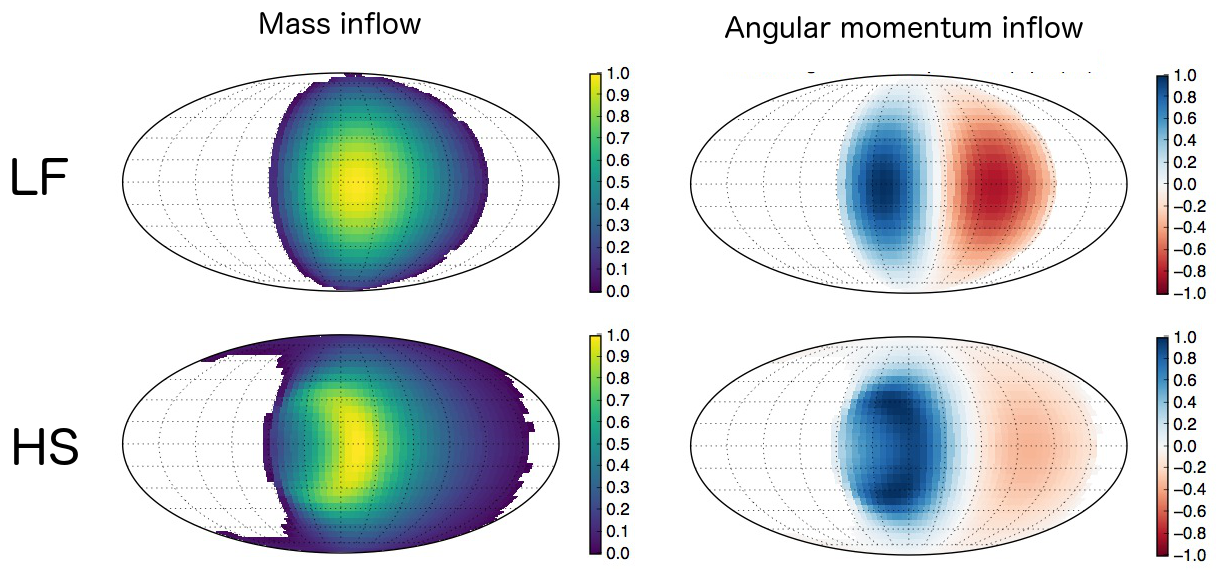
\includegraphics[width=2\columnwidth]{Pictures/inflow_maps.png}
\caption{Mollweide projections of local mass and angular momentum inflows within the simulation space centered on the accretor (dashed green sphere on Figure\ref{fig:big_picture}). The upper row corresponds to the light fast (LF) case while the bottom row is for the heavy slow (HS) case. Each map is scaled to its maximum (absolute) value and centered on the axis from the accretor to the donor star. Positive (resp. negative) values of angular momentum stands for locally prograde (resp. retrograde) flow with respect to the orbital motion.}
\label{fig:inflow_maps}
\end{figure*} 

% - - - - - - - - - - - - - - - - - - - - - - - - 
\subsection{Flow morphology}
\label{sec:morph}
% - - - - - - - - - - - - - - - - - - - - - - - - 

\subsubsection{Without cooling}
\label{sec:cool_F}

\subsubsection{With cooling}
\label{sec:cool_T}

FOR BLACK HOLES :
Presence of a disc-like structure which does not extend as far as in RLOF-fed systems (~LMXB) => no hysteresis in hardness-intensity diagram (for Cyg X-1, LMC X-1 or LMC X-3, the 3 wind-fed BH-HMXB). Indeed, the soft state might originate from : "A drop in the accretion rate affecting both flows would propagate through the halo immediately but might take up to several weeks to propagate through the disk.While the inner halo is thus temporarily depleted compared to the disk, a temporary soft state is expected." but if the disc has a much smaller outer radius (due to a much smaller angular momentum of the inflow), the viscous delay is expected to be so small that the dimming of the disc will be almost as fast as the one of the disc. \citep{Smith2002}. Explains also why no large outburst (ie a low contrast between the brightest and dimmest X-ray emission) in Cygnus X-1 (~x3) \citep{Grinberg:2014ux} : without an outer cool disc, the thermal instability resulting from the ionization of Hydrogen cannot occur (REF?). No quiescent state in Cyg X-1 : it is an argument in favor of the existence of a cool disc in the hard state.

% - - - - - - - - - - - - - - - - - - - - - - - - 
\subsection{Mass and angular momentum accretion rates}
\label{sec:mdot_ldot}
% - - - - - - - - - - - - - - - - - - - - - - - - 


% - - - - - - - - - - - - - - - - - - - - - - - - 
\subsection{Disc mass and morphology}
\label{sec:disc}
% - - - - - - - - - - - - - - - - - - - - - - - -

% ------------------------------------------------
\section{Conclusion}
\label{sec:conc}
% ------------------------------------------------


% ------------------------------------------------
\section*{Acknowledgments}
% ------------------------------------------------

% The authors are indebted to the anonymous referee who brought up several insightful questions and helped to improve this paper.

IEM has received funding from the Research Foundation Flanders (FWO) and the European Union's Horizon 2020 research and innovation program under the Marie Sk\l odowska-Curie grant agreement No 665501. IEM and JOS are grateful for the hospitality of the International Space Science Institute (ISSI), Bern, Switzerland which sponsored a team meeting initiating a tighter collaboration between massive stars wind and X-ray binaries communities. IEM also thanks Peter Kretschmar, Victoria Grinberg and Felix F\"urst for the fruitful discussions and the relevant comments they made on the present work. The simulations were conducted on the Tier-1 VSC (Flemish Supercomputer Center funded by Hercules foundation and Flemish government).


%%%%%%%%%%%%%%%%%%%%%%%%%%%%%%%%%%%%%%%%%%%%%%%%%%

%%%%%%%%%%%%%%%%%%%% REFERENCES %%%%%%%%%%%%%%%%%%

\bibliographystyle{agsm}
\begin{tiny}
\bibliography{/Users/Ileyk/Documents/Bibtex/article_sheared_wind_no_url}
\end{tiny}

%%%%%%%%%%%%%%%%%%%%%%%%%%%%%%%%%%%%%%%%%%%%%%%%%%


% Don't change these lines
\bsp	% typesetting comment
\label{lastpage}
\end{document}